\documentclass{report}
\usepackage[a4paper]{geometry}
\usepackage{amsmath}
\usepackage{bm}
\usepackage{pgfplots}
\usepackage{ amssymb }
\usepackage{color, soul}
\usepackage[backend=biber]{biblatex}
\addbibresource{references.bib}
\graphicspath{{images/}}


%opening
\title{Directed Study Report\\CSE4DIR}
\author{Ash Hall\\17756156}

\newcommand{\TODO}[1]{\sethlcolor{pink}\hl{\\(#1)\\}}
\newcommand{\FEEDBACK}[1]{\sethlcolor{green}\hl{\\ Feedback: \\#1\\}}
\newcommand{\TOCITE}[2][citation needed]{\textsuperscript{\underline{#1}}}
\newcommand{\SCORE}[2]{
	\begin{align*}
	\text{Score}_S &= #1 \\
	\text{Score}_T &= #2 \\
	\end{align*}
}

\begin{document}

	\begin{titlepage}
		\begin{center}
			\vspace*{5cm}


			{\huge \textbf{Directed Study Report}} \\
			\vspace{0.1cm}
			{\Large CSE4DIR} \\
			\vspace{0.3cm}
			{\large Investigation of Catastrophic Forgetting in Neural Networks} \\
			\vspace*{2cm}
			\textbf{Author} \\
			\textit{Ash Hall} \\
			Honours Student \\
			Department of Computer Science \\
			La Trobe University \\		
			\vspace{0.75cm}
			
			\textbf{Supervisor} \\
			\textit{Zhen He} \\
			Professor \\
			Department of Computer Science \\
			La Trobe University \\
			
			
			\vfill
		\end{center}
	\end{titlepage}
	\thispagestyle{empty}
	\newpage
	\thispagestyle{empty}
	\tableofcontents
	\thispagestyle{empty}
	\listoffigures
	\newpage
	\thispagestyle{empty}
	\newpage
	
	\setcounter{chapter}{1}	
	\chapter*{Directed Study Report}

	\section{Introduction}
	The purpose of this report is to investigate the effects of catastrophic forgetting in artificial neural networks. We will briefly discuss what catastrophic forgetting is and why it occurs, consider some approaches for minimising its effects, then present our experimental findings and discuss the results. \par \par
	As a neural network is improved by optimising the parameters on a per-example basis, they rapidly forget past learned knowledge to ``make way'' for new information. This purportedly occurs due to overlap in internal representations of new and old tasks, where a model may ``re-purpose'' important parameters for a new task, regardless of their importance for old tasks. While catastrophic forgetting is well recognised, its effects are yet to be quantified for comparison. We aim to produce empirical measurements by way of experimentation, and to provide a clear measure of the severity of catastrophic forgetting in artificial neural networks that can be used for comparison moving forward. \par
	
	\section{Transfer Learning}
	The training of a neural network occurs by presenting many examples, and iteratively optimising the weights. A dataset consisting of a small number of examples may be prohibitive to optimisation in this manner, as a model would likely over-fit to the training examples, and not be capable of generalising to novel examples. \emph{Transfer learning} minimising this problem, by allowing a pre-trained model to be re-purposed to a different dataset. \par
	The bulk of an image-classification neural network acts as a \emph{feature-extractor}, with studies\parencite{extractors} showing that a sufficiently-large image dataset leads to a highly-generalisable feature extractor. Transfer learning takes advantage of this property by taking the resultant feature extractor and amending the tail of a neural network to perform classification between different classes. Figure \ref{fig:transferlearning:1} shows a model pre-trained on a large image dataset being adapted to another. \par
	\begin{figure}[h]
		\centering
		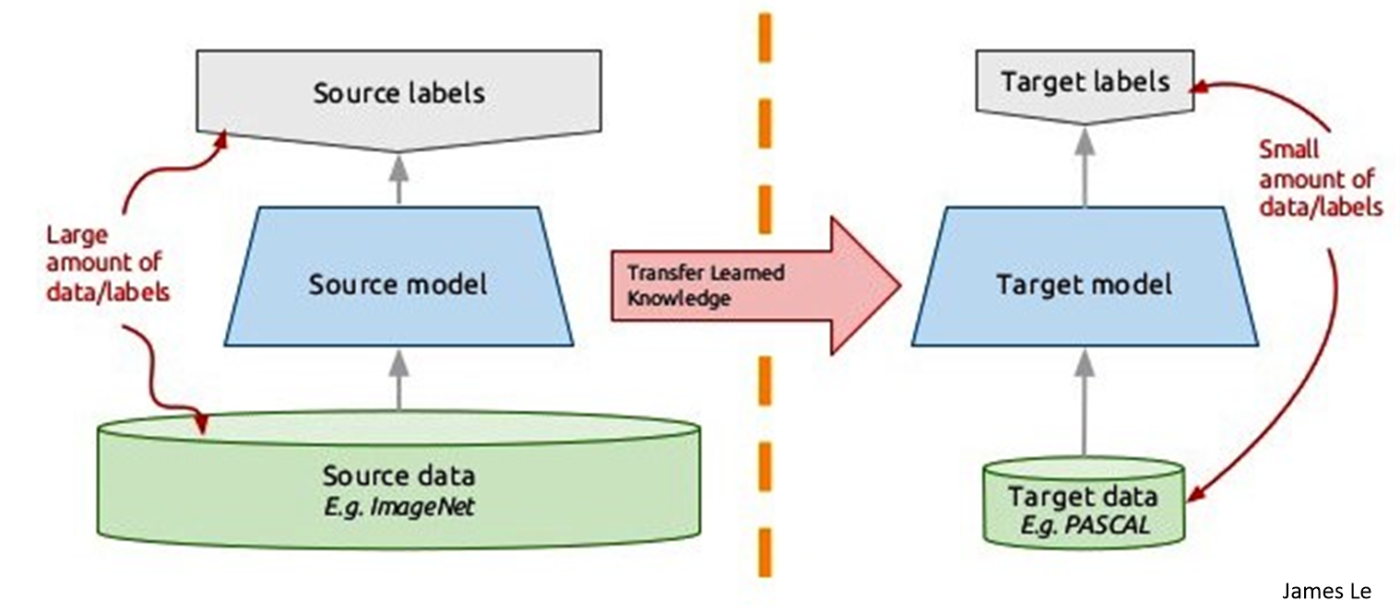
\includegraphics[width=11cm]{transferlearning}
		\caption{Transfer learning overview}
		\label{fig:transferlearning:1}
	\end{figure}
	There are two fundamental problems with this approach. The first is that although this lessens the effects of over-fitting, it doesn't entirely avoid them; training on a very small dataset is still prone to this problem. The other issue is that if you wished to not replace the old dataset classes, but add the new dataset classes to the model, you would need to store examples and repeatedly present them to the network during re-training. This introduces a whole suite of problems including training-example balancing, which we won't address here. \par
	Simply put, while providing strong results, transfer learning is limited in its usability, and is inherently inapplicable to the task of continuous learning -- which we'll address in the following section. \par
	
	\section{Continuous Learning}
	The tendency of neural networks to forget older information is known as catastrophic forgetting; the task of learning from a stream of new information a minimal amount of forgetting is known as continuous learning. \par
	Continuous learning differs from transfer learning in that in order to add classes to an image classifier using transfer learning, examples from the existing classes would need to be \emph{replayed} to the model over time, to ensure that it loses minimal performance on them. A condition of ``true'' continuous learning is that old examples need not be seen again -- this is a reasonable desire, as it would require an increasing amount of training time proportionate to the growing number of images and classes in a dataset. \par

	\subsection{Related Works}
	We will briefly discuss some works related to the task of mitigating catastrophic forgetting -- continuous learning. Although this report is to investigate the effects of catastrophic forgetting and not a survey of related work, it is good to consider other approaches. The following works were built to specifically target catastrophic forgetting, so serve as good points of reference. \par
	
	\subsubsection{Learning to Learn with Backpropagation of Hebbian Plasticity}
	The work by Miconi et. al. \parencite{hebbian} considers an observed biological neurological pattern, where synaptic efficacy (neuron firing strength) increases through persistent stimulation. In this approach, they define a ``Hebbian trace'', which acts as a moving-average of pair-wise synaptic activities. They train a plasticity parameter which determines how much the Hebbian trace affects a pair's connection. \par
	A network gains additional learning capacity by using this technique, as the network learns a sparser internal representation, effectively endowing a larger capacity for knowledge. Although catastrophic forgetting is somewhat reduced, this is not an ideal situation as the models internal capacity remains fixed and as such, is limited to the initial design. \par
	
	\subsubsection{Learning Without Forgetting}
	The technique proposed by Li et. al. \parencite{lwf} seeks to preserve acquired knowledge by recording the existing model's response to new classes examples. They augment the model by adding an additional set of outputs for the new classes, and producing a prediction probability distribution on the old heads using new class examples (figure \ref{fig:lwf:1}). \par
	\begin{figure}[h]
		\centering
		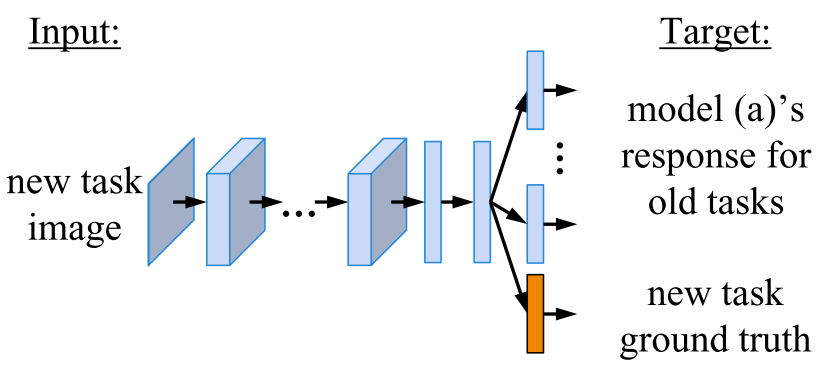
\includegraphics[width=8cm]{lwfarchitecture}
		\caption{Learning Without Forgetting architecture}
		A new output head (orange) is added for each batch of new classes. The model's predicted class probability distribution over the old classes is recorded and incorporated into the loss function. 
		\label{fig:lwf:1}
	\end{figure}
	This is a very literal and largely successful approach to mitigating catastrophic forgetting, but comes with a price -- the user of the model must know prior to performing inference which set of classes the image belongs to. This effectively makes it quite similar to having multiple models, the only difference being that the class groups share a feature extractor. \par

	\subsubsection{Overcoming Catastrophic Forgetting}
	The approach presented by Kirkpatrick et. al. \parencite{lwf} introduces a specialised loss function named \emph{elastic weight consolidation} (EWC), with the sole purpose of preserving old information. They compute a Fischer information matrix -- which is essentially a representation of each weight's importance for the pre-existing classes -- and use it to add an extra term to the loss calculation. With this term included, the loss function has the effect of restraining important parameters to a location in weight-space which provide good performance on the pre-existing classes. \par
	Similarly to \emph{Learning Without Forgetting}, this is an effective technique due to the fact that the retention of knowledge is explicitly embedded in the network's training. \par
	\par
	
	\subsubsection{Summary}
	The aforementioned techniques are designed to minimise the effects of catastrophic forgetting, and each does so in an effective and reasonable manner. That being said, the results yielded by each are incompatible as there is no consistent method for measuring catastrophic forgetting when extending neural networks to more classes. We seek to perform experiments which provide a consistent, coherent basis by which to measure these effects. \par
	

	\section{Environment}
	The following experiments were performed on a computer running the UNIX operating system, with two 8GB Nvidia GTX 1080 graphics cards, a quad-core processor and 64GB of memory. The implementation of the experiments was written using the Python interface for Tensorflow\parencite{tensorflow}, Google's open-source computational framework. Furthermore, Deepmind's Sonnet\parencite{sonnet} was used to provide a simple interface for Tensorflow. The graphing and result logging was done using Tensorboard, a visualisation tool included with Tensorflow. \par
	
	\section{Dataset}
	The experiments described in this report were performed using CIFAR-100\parencite{cifar100}, a dataset consisting of 60,000 32x32 images in 100 classes with 600 images per class. While a small -- in terms of spatial size -- dataset, the 100 classes emulate real-world by having such varied classes as motorcycles, snakes and bottles. \par
	
	\section{Framework}
	The code-base for the experiments is provided in figure \ref{fig:framework:1}, which details a high-level overview of the Python class, module and directory structure. The \texttt{Trainer} trains models, and takes command-line flags to switch the training mode (used when re-training models in different manners). It is also responsible for session management, and writing variables and Tensorboard data to the \texttt{bin} directory. The \texttt{GraphBuilder} abstracts the graph-building operations away from the \texttt{Trainer}, to allow for a cleaner training script. It reads from a configuration \texttt{YAML} file stored in \texttt{configs}, and builds the appropriate \texttt{Model} and \texttt{Optimizer} as required. The data loading, partitioning and sampling is presented via a consistent interface in the \texttt{dataloader} package, with the dataset loaded being specified in the configuration file mentioned. \\
	\begin{figure}[h]
		\centering
		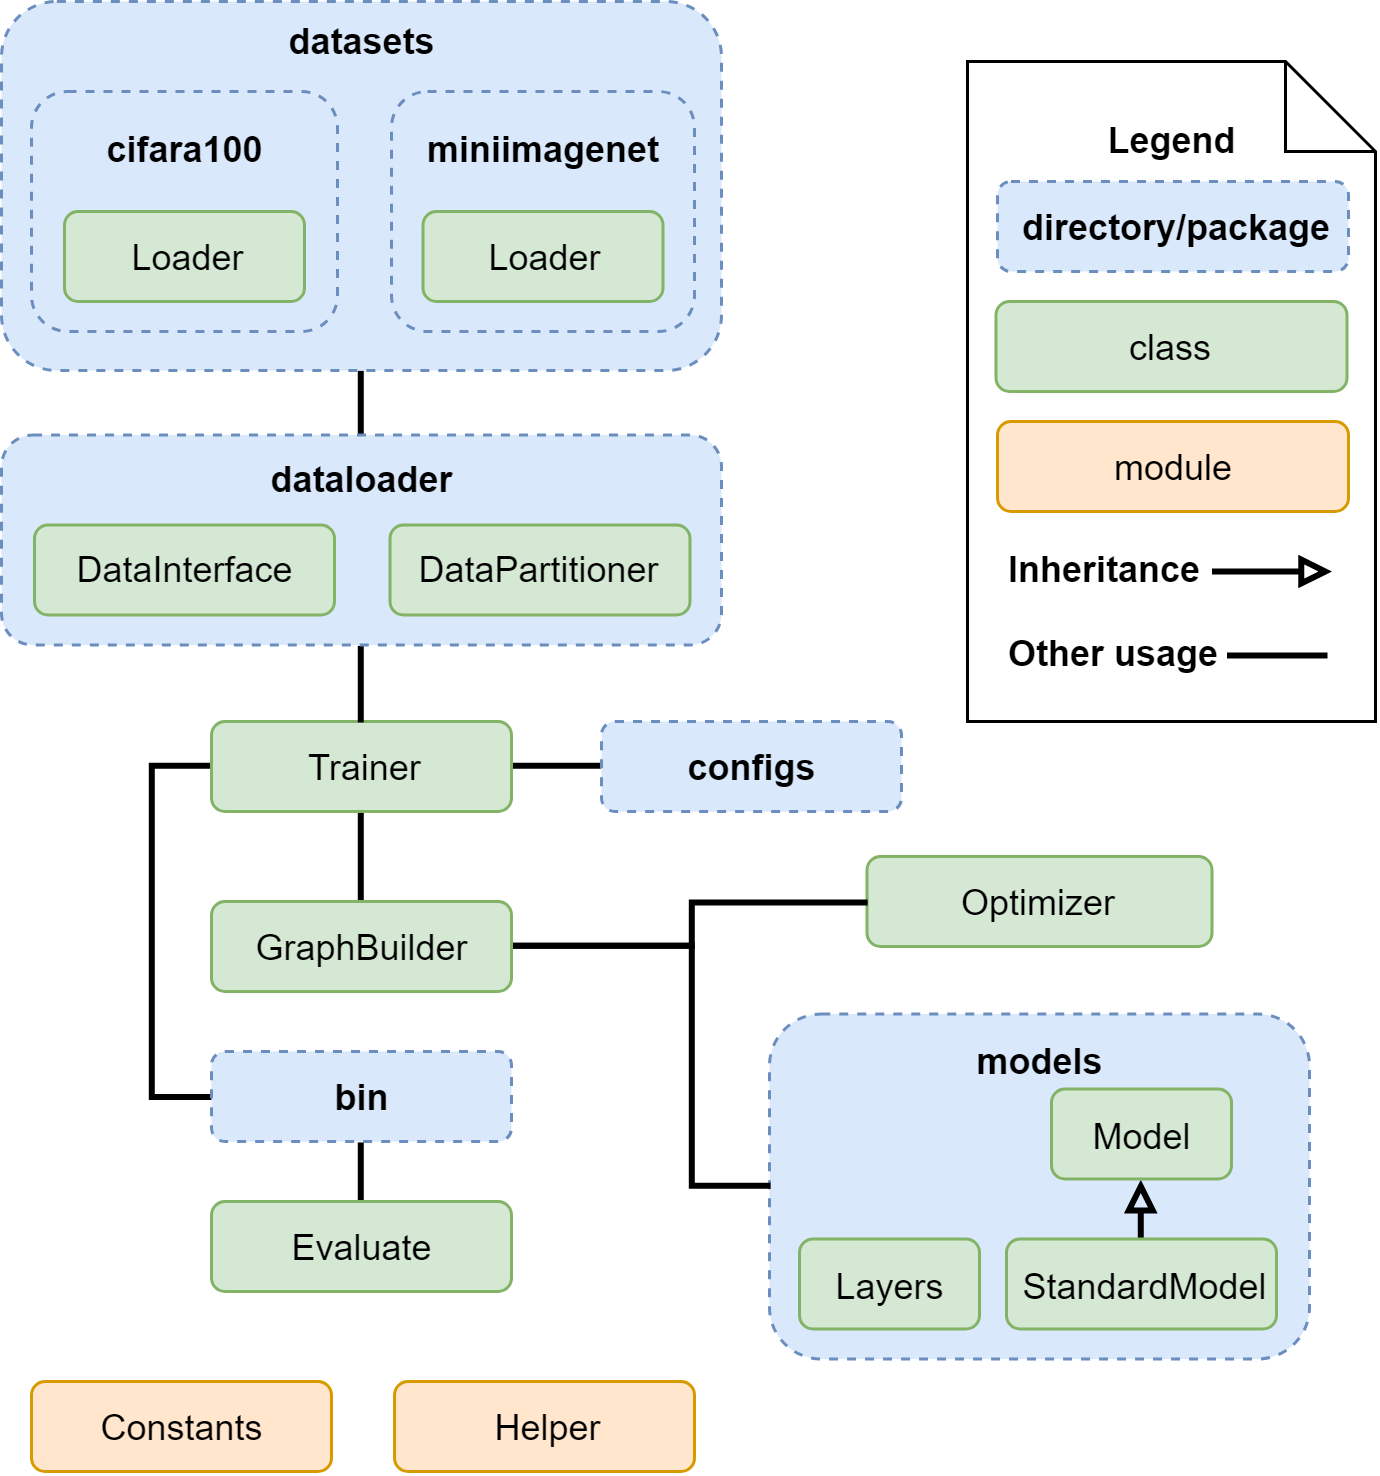
\includegraphics[width=11cm]{codeframework}
		\caption{Code-base Framework}
		A high-level view of the code-base structure. 
		\label{fig:framework:1}
	\end{figure}
	The described modular design provides the ability to quickly perform experiments with different datasets/model configurations. Automatic file-naming in the \texttt{bin} directory allows for experiment results to be easily reviewed and compared in Tensorboard with little effort. \par
	
	\section{Key Terminology}
	\textit{Source classes} refer to a set of classes on which a \textit{source model} has been pre-trained. Similarly, a \textit{target model} is produced by extending a source model's classification ability to also include a set of \textit{target classes} -- a disjoint set of classes to those that the source model was trained on. \par
	
	\section{Pre-Training Procedure} \label{pretrain}
	Each of the experiments were performed in a two-stage training procedure. The first stage of training was consistent for each experiment, which will now be described. \par
	The model architecture (figure \ref{fig:model:1}) used for training was consistent with other works of the same nature, with a body consisting of four convolutional blocks (figure \ref{fig:convblock:1}) followed by two parallel fully-connected output layers -- one each for the source target datasets. \par
	\begin{figure}[h]
		\centering
		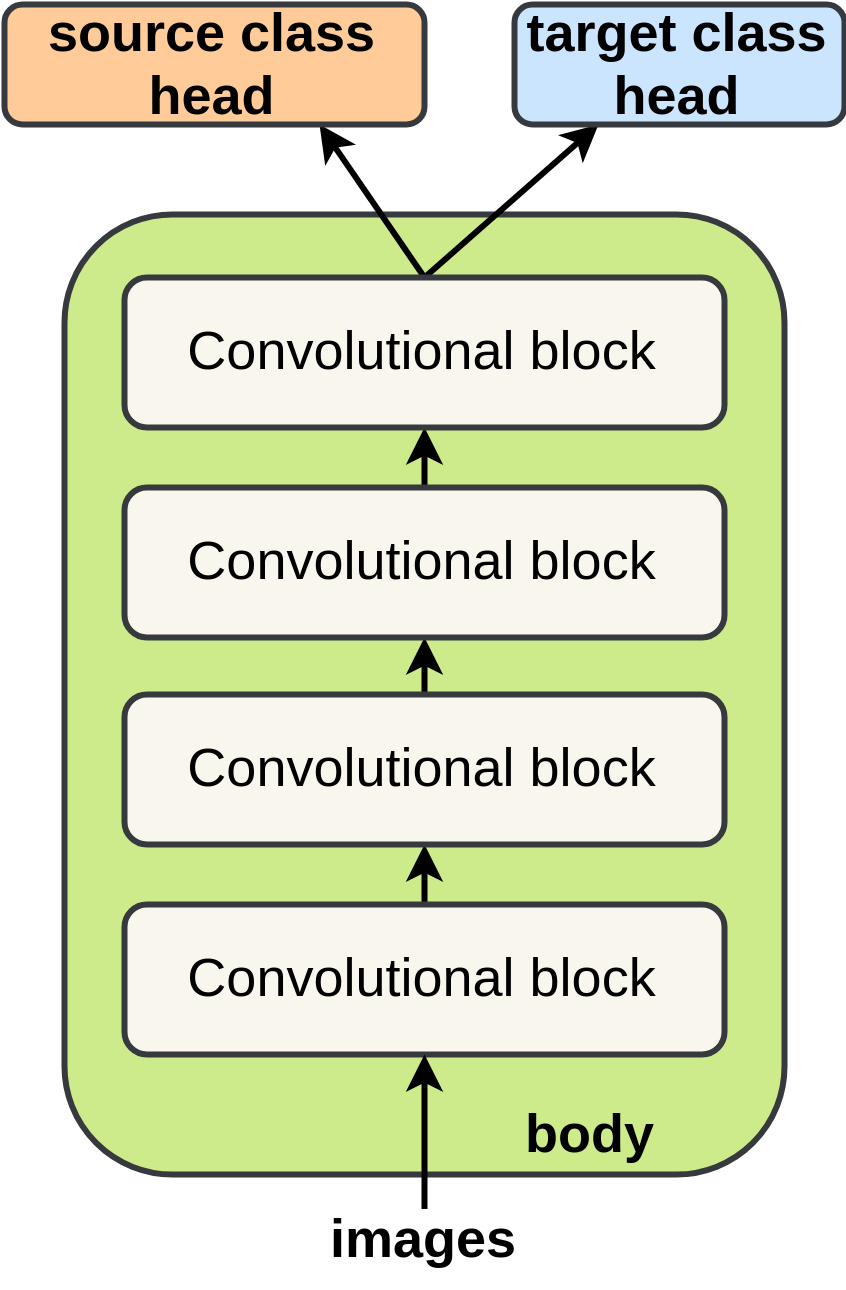
\includegraphics[width=4cm]{modelarchitecture}
		\caption{Model architecture}
		\label{fig:model:1}
		A separate fully-connected layer was used for each set of output classes
	\end{figure}
	\begin{figure}[h]
		\centering
		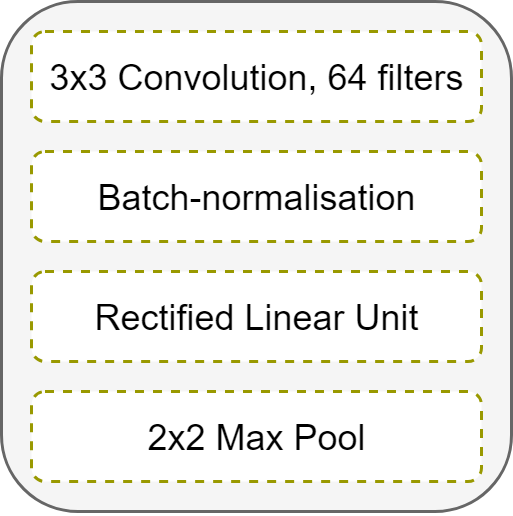
\includegraphics[width=3.5cm]{convblock}
		\caption{A convolutional block}
		\label{fig:convblock:1}
	\end{figure}
	For CIFAR-100, the number of total classes $N=100$, allowing us the ability to choose a smaller number of \emph{source} and \emph{target} classes and compare results. For a number of per-model source classes $N_S$, we can easily build $N-N_S-1$ overlapping incremental class subsets (figure \ref{fig:subsets:1}). \par
	We have chosen to work with the number of source classes $N_S = 50$, and the number of target classes $N_T = 10$, for a total of 60-way classifier in the end. This number of classes was chosen as the number of examples in each class is quite low, so training on 50 classes allows for the learning of somewhat general features. This is also to better simulate a real-world use-case, where classifiers in practice often have a large number of classes between which to predict. \par
	For each of these subsets, a model was trained using an Adam optimizer with a learning rate of $10^{-4}$. Due to the relatively small number of examples in the training/validation sets (500/100), training was stopped after 3000 iterations. Stopping at this many training iterations was determined empirically, as training for longer caused the model's performance on the validation set to drop due to over-fitting to the training set. \par
	The weights of each model were saved to disk and not modified any further, such that each experiment began with the exact same models. \par
	\begin{figure}[h]
		\centering
		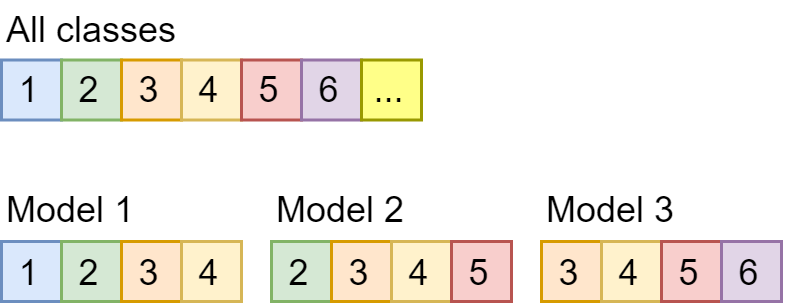
\includegraphics[width=8cm]{modelsubsets}
		\caption{Class subset selection}
		A number of class subsets can easily be selected using an overlapping, incremental selection schema. Example using number of source classes $N_S = 4$.
		\label{fig:subsets:1}
	\end{figure}

	\section{Metrics}
	A critical aspect is that the metrics reported are truly representative of the amount of catastrophic forgetting occurring. Due to this, each reported value is the average value over $N-N_S-1$ models. \par
	The quality of a model is measured by two components: the accuracy of the target model on the target classes, and the accuracy of the target model on the source classes. The former is a measure of how much the model learns about the target classes; the latter a measure of how much the model retains accuracy on the source classes. Instead of considering the precision in terms of their absolute value, we will instead compute the difference between target model and source model precision. Concretely, for a collection of images, a model will produce a number of correct (C) and incorrect (I) predictions. We can therefore compute the precision for a given model $\bm{\theta}$ on images $\bm{x}$ as in equation \ref{eqn:evaluation:1}.
	\begin{align} \label{eqn:evaluation:1}
	\text{Precision}(\bm{\theta}, \bm{x}) &= \frac{C}{C+I}
	\end{align}
	To compute the relative improvement or deterioration of performance of a model, we simply need to compute the difference in precision between a source model and corresponding target model. It is not possible to measure the source model's performance on the target classes however, as it is in the problem definition that the source model has never seen the target images. In this case, we will consider the source model precision on the source images as a de-facto baseline by which to measure the target model's performance on the target classes. The improvement score equations for source and target classes are shown in equations \ref{eqn:evaluation:2} and \ref{eqn:evaluation:3}, respectively.
	\begin{align} \label{eqn:evaluation:2}
	\text{Score}_S &= \text{Precision}(\bm{\theta}_T, \bm{x}_S) - \text{Precision}(\bm{\theta}_S, \bm{x}_S) \\
	\label{eqn:evaluation:3}
	\text{Score}_T &= \text{Precision}(\bm{\theta}_T, \bm{x}_T) - \text{Precision}(\bm{\theta}_S, \bm{x}_S)
	\end{align}
	By only considering the relative improvement of a model's performance, we don't allow the difficulty of the particular classes to distort our metrics, nor the quality of the source models. \par
	A positive score implies that the model has learnt from its experience, whereas a negative score implies that the model has forgotten. \par
	
	\section{Experiments and Results}
	After training a batch of 51 models as according to section \ref{pretrain}, the results obtained on the validation set of the source dataset $\bm{x}_T$ was 38.87\%. \par
	While this may seem like a low validation accuracy, it is worth mentioning that this 50-way classification task is already quite difficult, given that there are only $500+100=600$ images available for each image. The task of generalising from 500 known to 100 previously unseen examples is difficult, with other works typically employing image-augmentation techniques such as rotations, flips, crops, etc. No image augmentation techniques were used for this result, so that we may consider only the ``true'' classification accuracy. \par
	
	\subsection{Retraining with Source and Target Datasets}
	This experiment explores the performance under ideal circumstances -- that is, where training can occur using images from both the source and target dataset. Having access to the source dataset minimises the effects of catastrophic forgetting, as models are consistently exposed to examples from the source dataset. It is unfair to compare the results from this experiment with those from other experiments, so this simply provides the ``best possible'' results. \par
	After training for 1000 iterations, the classification accuracy on the source and target datasets were 37.21\% and 27.42\%, respectively -- resulting in scores:
	\SCORE{-0.017}{-0.115}
	
	It is reasonable to expect a negative score for the source dataset, as simply by increasing the number of classes from 50 to 60 there is an inherent drop in accuracy. While the model did learn to some extent to classify between the target classes, its performance is quite poor. There are many factors which affect this, but likely it is due to the fact that the weights were already well-refined to the source classes' distributions, making it hard for the model to transfer its knowledge to the new classes. As we'll see later on, relieving the model of its duty to classify the source classes allows the it to better utilise its representational power to learn the target classification task. \par

	\subsection{Retraining with only Target Dataset}
	The following experiments actually investigate the effects of catastrophic forgetting, as models aren't exposed to the source dataset after pre-training is complete. The techniques employed in this section is referred to as ``parameter freezing'', which is performed by simply locking parameters for certain parts of the model, now allowing them to change when re-training. \par 
	We will explore the effects of different ``freezing strategies'' by re-training the models with different sections of the models frozen (figure \ref{fig:freezing:1}), and will discuss the purpose behind the different freezing strategies and their consequences. \par
	Catastrophic forgetting has a rapid onset, which can be seen in figure \ref{fig:book:1}, reporting the score at retraining steps 5, 10, 20 and 50. The final scores are compared in \ref{fig:book:2}, where we see that the third freezing strategy produces the best results, but that no techniques satisfactorily mitigate the effects of catastrophic forgetting. \par
	
	\begin{figure}[h]
		\centering
		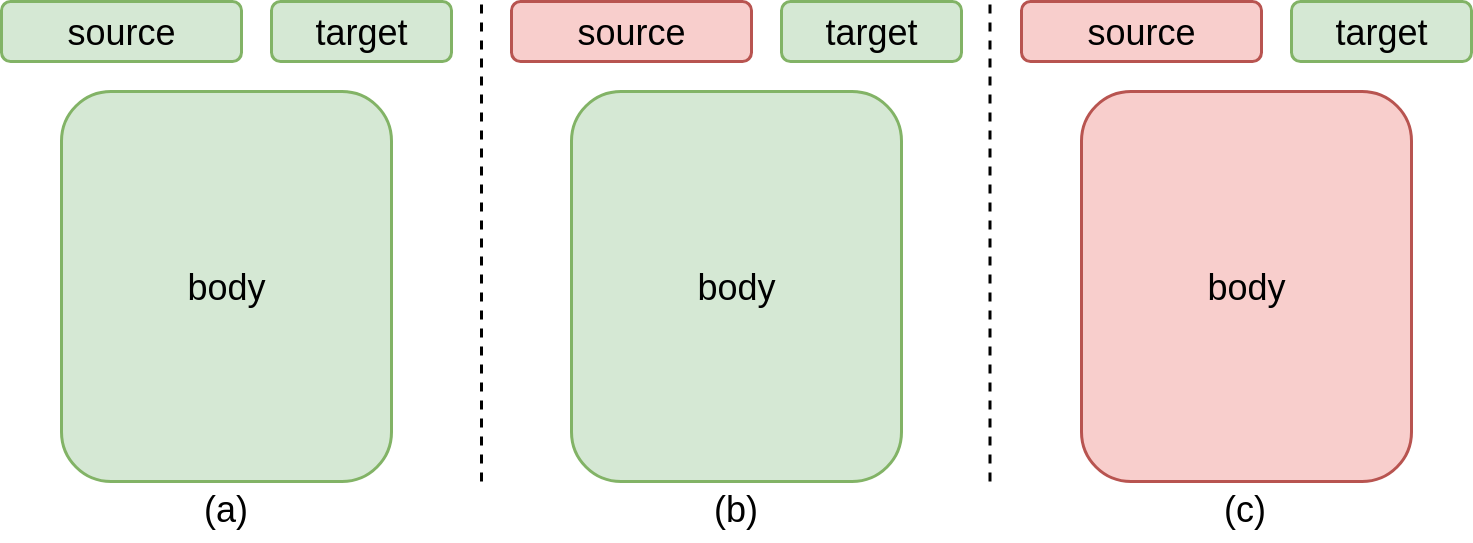
\includegraphics[width=10cm]{freezing}
		\caption{Retraining freezing strategies}
		The strategies used for weight-freezing when re-training. Green indicates trainable parameters, red indicates frozen parameters.
		\label{fig:freezing:1}
	\end{figure}
	\subsubsection{Training All Weights}
	In this experiment we consider the most naive of re-training strategies -- re-training the entire model with no consideration for frozen weights. We should expect that the source output head's predictions quickly go to zero, as the ``correct answer'' is to never one of those classes. Training for 50 iterations yielded scores of:
	\SCORE{-0.389}{0.128}
	Catastrophic forgetting occurred very quickly and with great effect, with the model's performance on the source classes dropping essentially to zero. This is to be expected and is a typical demonstration of catastrophic forgetting, as there is no attempt made to mitigate its effects. The model's body -- which is supposed to act as a general feature-extractor -- quickly discards information learnt relating to the source classes to learn quickly about the new classes. \par
	
	\subsubsection{Training Body and Target Output Head}
	This experiment investigates only freezing the source class output head. We shouldn't expect this to perform very well, as although we aren't \emph{explicitly} training the source output head to never produce high probabilities, the target output head may learn to produce very high confidence in its predictions to ``outweigh'' the source output head. Training for 50 iterations yielded scores of:
	\SCORE{-0.389}{0.126}
	The results were very similar to those of the previous experiment, as we expected. The reason this is occurring is that not only is the target head outweighing the source head's predictions, the features in the body are still being changed. The output head of a neural network classifier can be considered a representation of the intensity to which a particular feature appears for a given class. We are now modifying what each feature actually is, but not allowing the source head to update its representation to match them. \par
	
	\subsubsection{Training only Target Output Head}
	What we now explore is the method regularly used in transfer learning, where only the new output head (the target output head) has its parameters changed. This differs slightly to transfer learning, in that transfer learning implies that the original head is removed entirely. We can expect that this technique will minimise catastrophic forgetting the most, as neither the feature extractor nor the source output head have their weights shifted. After training for 50 iterations, the model produced the scores:
	\SCORE{-0.27}{-0.204}
	As this is the result with the least forgetting thus far, trained for longer to view the best possible results. After 2500 iterations, we had:
	\SCORE{-0.385}{0.164}
	As expected, the catastrophic forgetting took much longer to occur to such an extent as previously encountered. However, after training for longer the model yielded its best target score yet - the accuracy produced is significantly higher than the accuracy on the source set during pre-training.\par
	The model's accuracy on the target validation set was approximately the same as on the target training set, which means that there was practically no over-fitting on the training set after so many iterations. This result is interesting, as we should expect that extensive training results in over-fitting just as we discussed in section \ref{pretrain}. We theorise that this occurred due to a very limited amount of changes that the network could apply in order to improve. The body could be modified during training in other experiments, resulting in a feature extractor that is tightly-bound to the images it has seen. In contrast, this training schema only allows for adjustments to the output head, meaning that the model has to find the best-possible combination of features to represent the classes. \par
	In only having access to modify the output head, the model is very limited in its fitting capacity, resulting in a generalised representation of the target classes. \par
	\begin{figure}[h]
		\centering
		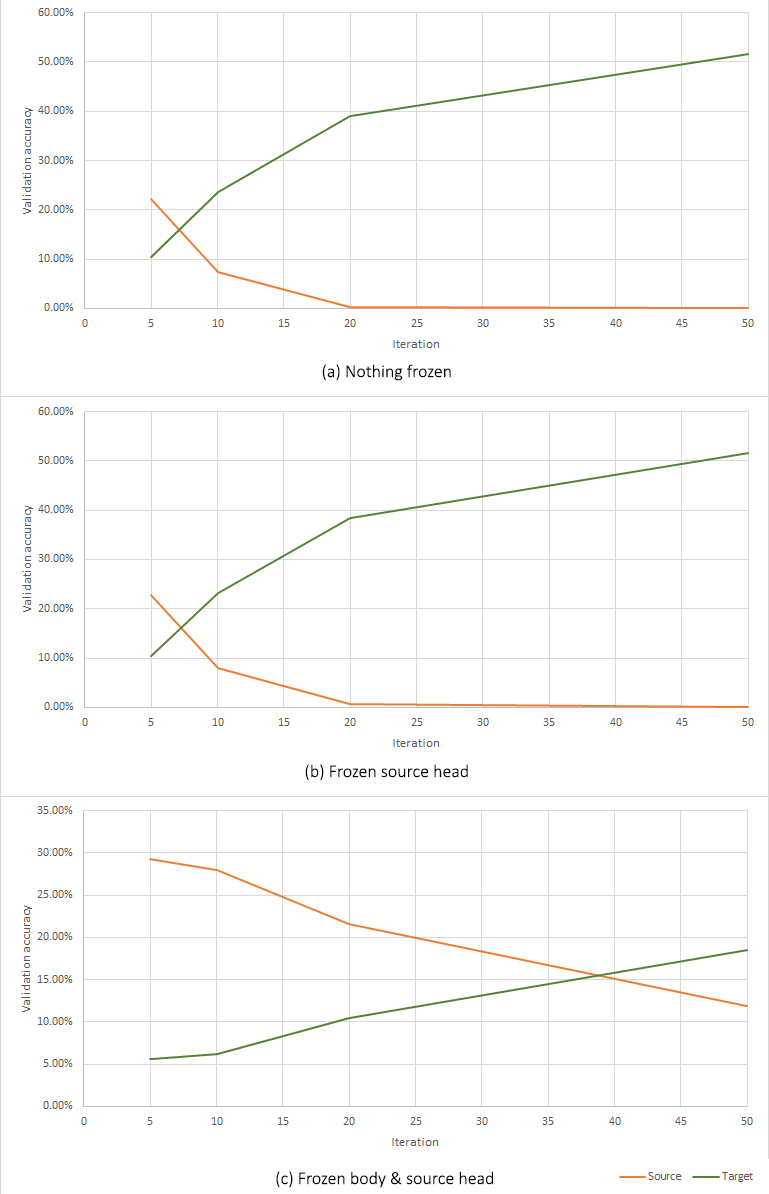
\includegraphics[width=12cm]{book}
		\caption{Freezing strategy learning/forgetting rates}
		\label{fig:book:1}
	\end{figure}

	\begin{figure}[h]
		\centering
		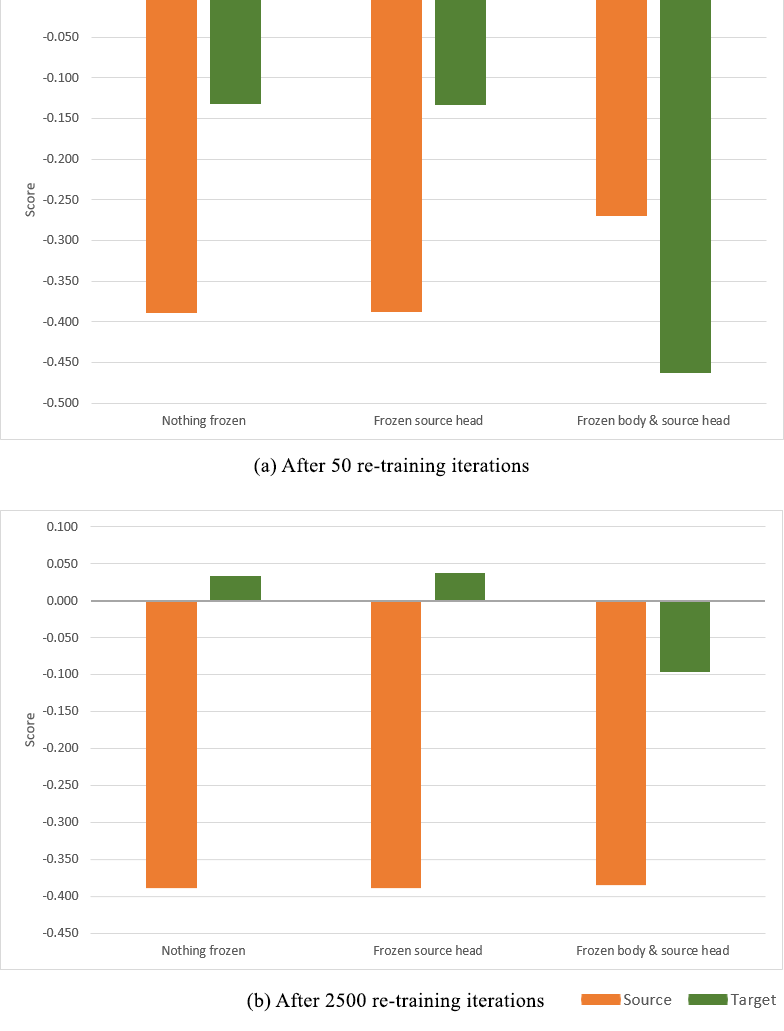
\includegraphics[width=12cm]{book2}
		\caption{Freezing strategy learning/forgetting scores}
		A comparison of results showing the scores for each freezing strategy.
		\label{fig:book:2}
	\end{figure}

		
	\section{Summary}
	We have explored different weight-freezing strategies to minimise the effects of catastrophic forgetting, and have explored the severity to which catastrophic forgetting occurs when re-training a neural network. We found no satisfactory method for catastrophic forgetting. The effect is slowed if only retraining the new output head, but learning is also, with no mid-point resulting in good classification results on both sets of classes. Although the resultant model did have good generalisation ability, exists a limit. The feature extractor already parametrised during the pre-training procedure is not guaranteed to represent the target classes, especially if the source and target classes differ by a large amount. \par	
	
\end{document}
